\documentclass[xcolor=svgnames,table]{beamer}
%\usepackage{movie15}
\usepackage{amsmath}
\usepackage{graphicx}
\usepackage{multimedia}
\usepackage{hyperref}
\usepackage{ifthen}
\usepackage{etex}
\usepackage{tikz} 
\usepackage{pgfplots}
\usepackage{filecontents}
\usepackage{xcolor}
\usepackage[]{algorithm2e}
\usepackage[font=footnotesize,labelformat=empty,
            justification=raggedright,
%            singlelinecheck=false
  ]{caption}
\usetikzlibrary{scopes}
\usetikzlibrary{arrows}
\usetikzlibrary{arrows.meta}
\usetikzlibrary{patterns}
\usetikzlibrary{bayesnet}

\usetikzlibrary{arrows}
\usetikzlibrary{shapes,arrows,chains}
\usetikzlibrary{intersections}
\usetikzlibrary[calc]

\tikzstyle{solidarrow} = [arrows={-Stealth[length=8pt]}]
\tikzstyle{dashedarrow} = [solidarrow, dashed]
\tikzstyle{paramnode} = [circle, fill=black, scale=0.5]

\tikzset{mega thick/.style={line width=2pt}}

\tikzstyle{latent} = [circle,fill=white,draw=black,inner sep=1pt,
minimum size=25pt, font=\fontsize{10}{10}\selectfont, node distance=1]
% \tikzstyle{latentsmall} = [circle,fill=white,draw=black,inner sep=0pt,
%  minimum size=25pt, font=\fontsize{5}{5}\selectfont, node distance=1]
\tikzstyle{latentsmall} = [latent]

\tikzstyle{platecaptionnoposition} = [caption, node distance=0, inner sep=0pt]
\tikzstyle{topright} = [platecaptionnoposition, above left=5pt and 0pt of #1.north east] 
\tikzstyle{bottomright} = [platecaptionnoposition, below left=5pt and 0pt of #1.south east] 

% \plateex [options] {name} {fitlist} {position} {caption}
\newcommand{\plateex}[5][]{ %
	\node[wrap=#3] (#2-wrap) {}; %
	\node[#4=#2-wrap] (#2-caption) {#5}; % 
	\node[plate=(#2-wrap)(#2-caption), #1] (#2) {}; %
}

% \edgeex [options] {inputs} {outputs}
\newcommand{\edgeex}[3][solidarrow]{ %
	% Connect all nodes #2 to all nodes #3.
	\foreach \x in {#2} { %
		\foreach \y in {#3} { %
			\path (\x) edge [->,#1] (\y) ;%
			%\draw[->,#1] (\x) -- (\y) ;%
		} ;
	} ;
}


%%%%%%%%%%%%%%%%%%%%%%%%%%%%%%%%%%%%%%%%%%%%%%%%%%%%%%%%%%%%%%%%%%%%%%%%%%%%%%%%%%%%
\newcommand*{\colormapmin}{0}%
\newcommand*{\colormapmax}{1}%
\newcommand{\colored}[1]{%
  \pgfmathsetmacro\y{100.0*(#1-\colormapmin)/(\colormapmax-\colormapmin)}
  \edef\temp{\noexpand\cellcolor{green!\y!red!30!white}}\temp #1
}%

\tikzset{
    %Define standard arrow tip
    >=stealth',
    %Define style for boxes
    punkt/.style={
           rectangle,
           rounded corners,
           draw=black, very thick,
           text width=6.5em,
           minimum height=2em,
           text centered},
    % Define arrow style
    pil/.style={
           ->,
           thick,
           shorten <=2pt,
           shorten >=2pt,}
}

\newcommand{\ve}[1]{\mathbf{#1}}
\newcommand{\real}{\mathbb{R}}


\usetheme{Darmstadt}
\title{Estimating policy with Variational Bayes \\ without much pain}
\subtitle{}
\institute{Theoretical Neuroscience lab \\ Philipps-Universit\"{a}t Marburg}
\author[Dmytro Velychko]{Dmytro Velychko\\{\small Dr. Dominik Endres}}
\date{Last edited: \today}
\begin{document}

%%%%%%%%%%%%%%%%%%%%%%%%%%%%%%%%%%%%%%%%%%%%%%
\begin{frame}
\titlepage
\end{frame}	

%%%%%%%%%%%%%%%%%%%%%%%%%%%%%%%%%%%%%%%%%%%%%%
\begin{frame}{Overview}
\tableofcontents
\end{frame}

\section{Problem}

%%%%%%%%%%%%%%%%%%%%%%%%%%%%%%%%%%%%%%%%%%%%%%
\begin{frame}
\frametitle{Supervised policy estimation}
\begin{center}
\scalebox{0.5}{
  %\usetikzlibrary{bayesnet}
%\tikzstyle{solidarrow} = [arrows={-Stealth[length=8pt]}]
\tikzstyle{dashedarrow} = [solidarrow, dashed]
\tikzstyle{paramnode} = [circle, fill=black, scale=0.5]

\tikzset{mega thick/.style={line width=2pt}}

\tikzstyle{latent} = [circle,fill=white,draw=black,inner sep=1pt,
minimum size=25pt, font=\fontsize{10}{10}\selectfont, node distance=1]
% \tikzstyle{latentsmall} = [circle,fill=white,draw=black,inner sep=0pt,
%  minimum size=25pt, font=\fontsize{5}{5}\selectfont, node distance=1]
\tikzstyle{latentsmall} = [latent]

\tikzstyle{platecaptionnoposition} = [caption, node distance=0, inner sep=0pt]
\tikzstyle{topright} = [platecaptionnoposition, above left=5pt and 0pt of #1.north east] 
\tikzstyle{bottomright} = [platecaptionnoposition, below left=5pt and 0pt of #1.south east] 

% \plateex [options] {name} {fitlist} {position} {caption}
\newcommand{\plateex}[5][]{ %
	\node[wrap=#3] (#2-wrap) {}; %
	\node[#4=#2-wrap] (#2-caption) {#5}; % 
	\node[plate=(#2-wrap)(#2-caption), #1] (#2) {}; %
}

% \edgeex [options] {inputs} {outputs}
\newcommand{\edgeex}[3][solidarrow]{ %
	% Connect all nodes #2 to all nodes #3.
	\foreach \x in {#2} { %
		\foreach \y in {#3} { %
			\path (\x) edge [->,#1] (\y) ;%
			%\draw[->,#1] (\x) -- (\y) ;%
		} ;
	} ;
}

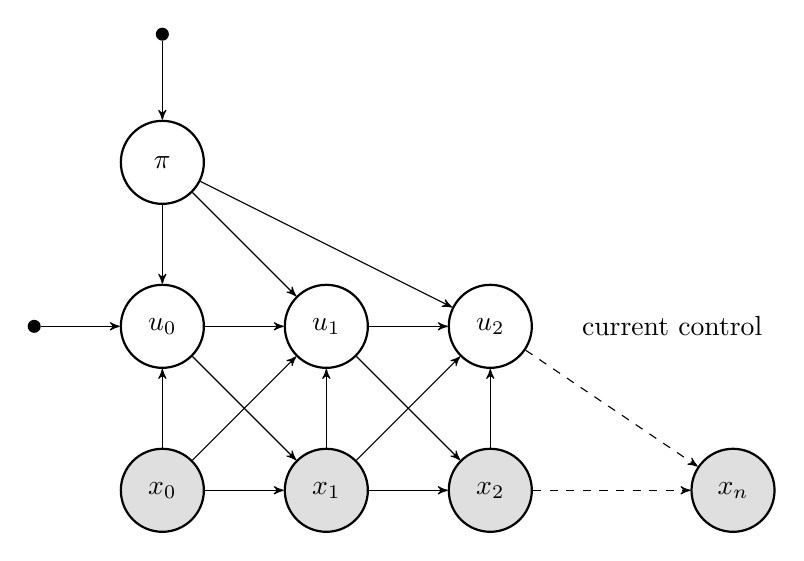
\begin{tikzpicture}

\tikzstyle{mylatent} = [circle,fill=white,draw=black,inner sep=1pt,
minimum size=30pt, thick]
\tikzstyle{myobs} = [circle,fill=gray!25,draw=black,inner sep=1pt,
minimum size=30pt, thick]

\node[mylatent] (u0) {$u_0$};
\node[mylatent, right=1 cm of u0] (u1) {$u_{1}$};
\node[mylatent, right=1 cm of u1] (u2) {$u_{2}$};
%\node[mylatent, right=2 cm of u2] (un) {$u_{n}$};

\node[myobs, below=1 cm of u0] (x0) {$x_0$};
\node[myobs, right=1 cm of x0] (x1) {$x_{1}$};
\node[myobs, right=1 cm of x1] (x2) {$x_{2}$};
\node[myobs, right=2 cm of x2] (xn) {$x_{n}$};

%\node[paramnode, left=1 cm of x0] (px0) {$$};
%\edge {px0} {x0}; 

\edge {x0} {x1};
\edge {x1} {x2}; 
\draw [dashed, ->] (x2) edge (xn);

\edge {u0} {x1}; 
\edge {u1} {x2}; 
\draw [dashed, ->] (u2) edge (xn);

\edge {x0} {u1}; 
\edge {x1} {u2}; 

\edge {u0} {u1}; 
\edge {u1} {u2}; 

\edge {x0} {u0}; 
\edge {x1} {u1}; 
\edge {x2} {u2}; 

\node[paramnode, left=1 cm of u0] (pu0) {$$};
\edge {pu0} {u0};

\node[mylatent, above=1 cm of u0] (policy) {$\pi$};

\edge {policy} {u0, u1, u2};

\node[paramnode, above=1 cm of policy] (ppolicy) {$$};
\edge {ppolicy} {policy};

\node [right=0.5cm of u2] {current control};

\end{tikzpicture}


}
\end{center}
Supervised learning of policy.\\
Full Bayesian treatment with Monte Carlo Variational Bayes.
\end{frame}


%%%%%%%%%%%%%%%%%%%%%%%%%%%%%%%%%%%%%%%%%%%%%%
\begin{frame}[fragile]{Why Bayesian? Bayesian Model Comparison}
Data $X$,  model $M_i$, parameters $\theta$
\begin{align}
    p(M_i | X) &= \frac{1}{Z_M} \int p(X | \theta, M_i) p(\theta | M_i,) p(M_i) d\theta \\
    \frac{p(M_a | X)}{p(M_b | X)} &= \frac{p(M_a) \int p(X | \theta, M_a) p(\theta | M_a)d\theta  }{p(M_b) \int p(X | \theta, M_b) p(\theta | M_b)d\theta} \\
    p(X | M_i) &= p(M_b) \int p(X | \theta, M_i) p(\theta | M_i)d\theta
\end{align}
\end{frame}




\section{Monte Carlo integration}





%%%%%%%%%%%%%%%%%%%%%%%%%%%%%%%%%%%%%%%%%%%%%%
\begin{frame}
\frametitle{Jensen's inequality}
\begin{center}
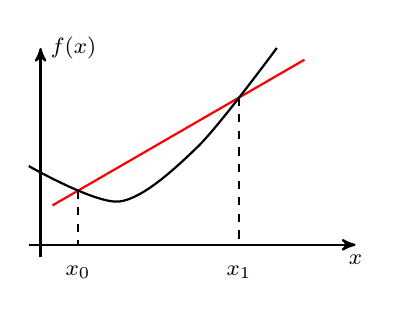
\begin{tikzpicture}[scale=0.5,
    thick,
    >=stealth']
\coordinate (O) at (0,0);
  \draw[->] (-0.3,0) -- (8,0) coordinate[label = {below:$x$}] (xmax);
  \draw[->] (0,-0.3) -- (0,5) coordinate[label = {right:$f(x)$}] (ymax);

  \draw[red, name path=x] (0.3,1.0) -- (6.7,4.7);
  \draw[name path=y] plot[smooth] coordinates {(-0.3,2) (2,1.1) (4,2.5) (6,5)};

  \scope[name intersections = {of = x and y, name = i}]
   \draw [dashed] (i-1) -- (i-1 |- O) node[label = {below:$x_0$}] {};
   \draw [dashed] (i-2) -- (i-2 |- O) node[label = {below:$x_1$}] {};
  \endscope
\end{tikzpicture}
\end{center}
\only<1> {
For any convex function $f$:
  \begin{align}
    f(E(X)) \leq E(f(X))
  \end{align}
}
\only<2> {
In integral form: 
\begin{align}
  f\left(\int g(x) p(x) dx \right) \leq \int f(g(x)) p(x) dx
\end{align}
}
For concave functions this inequality reverses
\end{frame}

%%%%%%%%%%%%%%%%%%%%%%%%%%%%%%%%%%%%%%%%%%%%%%
\begin{frame}[fragile]{Why Bayesian? Bayesian Model Comparison}
Data $X$,  model $M_i$, parameters $\theta$
\begin{align}
    p(M_i | X) &= \frac{1}{Z_M} \int p(X | \theta, M_i) p(\theta | M_i,) p(M_i) d\theta \\
    \frac{p(M_a | X)}{p(M_b | X)} &= \frac{p(M_a) \int p(X | \theta, M_a) p(\theta | M_a)d\theta  }{p(M_b) \int p(X | \theta, M_b) p(\theta | M_b)d\theta} \\
    p(X | M_i) &= p(M_b) \int p(X | \theta, M_i) p(\theta | M_i)d\theta
\end{align}
Using Jensen's inequality, for any model $M_i$:
\begin{align}
    p(X) &= \int p(X | \theta) p(\theta)d\theta \\
    p(X) &= \int p(X, \theta) d\theta = \exp \log \int q(\theta | X) \frac{p(X, \theta)}{q(\theta | X)} d\theta\\ 
    \log p(X) &\geq \int q(\theta | X) \log \frac{p(X, \theta)}{q(\theta | X)} d\theta = ELBO
\end{align}

\end{frame}

%%%%%%%%%%%%%%%%%%%%%%%%%%%%%%%%%%%%%%%%%%%%%%
\begin{frame}
\frametitle{Monte Carlo integration}
Evaluate the function we want to integrate in uniformly random positions to approximate the integral
\begin{align}
\int f(x) dx \approx \frac{1}{N} \sum_{i=1}^N f(\sigma_i)
\end{align}
Variance decreases with number of random points. Think of Bayesian evidence accumulaition.
\end{frame}

%%%%%%%%%%%%%%%%%%%%%%%%%%%%%%%%%%%%%%%%%%%%%%
\begin{frame}
\frametitle{Monte Carlo integration. Expectations}
Estimating an expectation:
\begin{align}
\sigma_i &\sim p(x) \\
\int f(x) p(x) dx &\approx \frac{1}{N} \sum_{i=1}^N f(\sigma_i)
\end{align}
What if we can't sample efficiently from p(x)? Use a simple distribution $q$, weight the samples
\begin{align}
\sigma_i &\sim q(x) \\
\int f(x) p(x) dx &\approx \frac{1}{N} \sum_{i=1}^N f(\sigma_i) \frac{p(\sigma_i)} {q(\sigma_i)}
\end{align}
\end{frame}

\section{Variational Bayes}
%%%%%%%%%%%%%%%%%%%%%%%%%%%%%%%%%%%%%%%%%%%%%%
\begin{frame}
\frametitle{Variational Bayes}
Recall: 
\begin{align}
    ELBO &= \int q(\theta | X) \log \frac{p(X, \theta)}{q(\theta | X)} d\theta \\
    &= \int q(\theta | X) \log p(X, \theta) d\theta - \int q(\theta | X) \log q(\theta | X) d\theta
\end{align}
We want to optimize ELBO w.r.t. parameters $\phi$ of $q_{\phi}(\theta | X)$
\begin{align}
    \frac{\partial ELBO}{\partial \phi} &= \frac{\partial}{\partial \phi} \left(  \int q(\theta | X) \log p(X, \theta) d\theta - \int q(\theta | X) \log q(\theta | X) d\theta \right) \\
    &\approx \frac{\partial}{\partial \phi} \frac{1}{N} \sum_{i=1}^N \left(  \log p(X, \theta_{\phi i}) - \log q(\theta_{\phi i} | X) \right) 
\end{align}

where $\theta_{\phi i} \sim q_{\phi}(\theta | X)$

\end{frame}

%%%%%%%%%%%%%%%%%%%%%%%%%%%%%%%%%%%%%%%%%%%%%%
\begin{frame}
\frametitle{Inference with MC Variational Bayes}

\begin{algorithm}[H]
 \KwData{observed data}
 \KwResult{variational parameters, ELBO}
 \Repeat{convergence}{
   Draw N samples from $q_{\phi}(\theta | X)$ \;
   Approximate ELBO with Monte Carlo integration \;
   Compute $\frac{\partial ELBO}{\partial \phi}$ \;
   update parameters $\phi$ \;
 }
\end{algorithm}
\end{frame}

\section{Policy estimation}



%%%%%%%%%%%%%%%%%%%%%%%%%%%%%%%%%%%%%%%%%%%%%%
\begin{frame}
\frametitle{Supervised policy estimation}
\begin{center}
\scalebox{0.5}{
  %\usetikzlibrary{bayesnet}
%\tikzstyle{solidarrow} = [arrows={-Stealth[length=8pt]}]
\tikzstyle{dashedarrow} = [solidarrow, dashed]
\tikzstyle{paramnode} = [circle, fill=black, scale=0.5]

\tikzset{mega thick/.style={line width=2pt}}

\tikzstyle{latent} = [circle,fill=white,draw=black,inner sep=1pt,
minimum size=25pt, font=\fontsize{10}{10}\selectfont, node distance=1]
% \tikzstyle{latentsmall} = [circle,fill=white,draw=black,inner sep=0pt,
%  minimum size=25pt, font=\fontsize{5}{5}\selectfont, node distance=1]
\tikzstyle{latentsmall} = [latent]

\tikzstyle{platecaptionnoposition} = [caption, node distance=0, inner sep=0pt]
\tikzstyle{topright} = [platecaptionnoposition, above left=5pt and 0pt of #1.north east] 
\tikzstyle{bottomright} = [platecaptionnoposition, below left=5pt and 0pt of #1.south east] 

% \plateex [options] {name} {fitlist} {position} {caption}
\newcommand{\plateex}[5][]{ %
	\node[wrap=#3] (#2-wrap) {}; %
	\node[#4=#2-wrap] (#2-caption) {#5}; % 
	\node[plate=(#2-wrap)(#2-caption), #1] (#2) {}; %
}

% \edgeex [options] {inputs} {outputs}
\newcommand{\edgeex}[3][solidarrow]{ %
	% Connect all nodes #2 to all nodes #3.
	\foreach \x in {#2} { %
		\foreach \y in {#3} { %
			\path (\x) edge [->,#1] (\y) ;%
			%\draw[->,#1] (\x) -- (\y) ;%
		} ;
	} ;
}

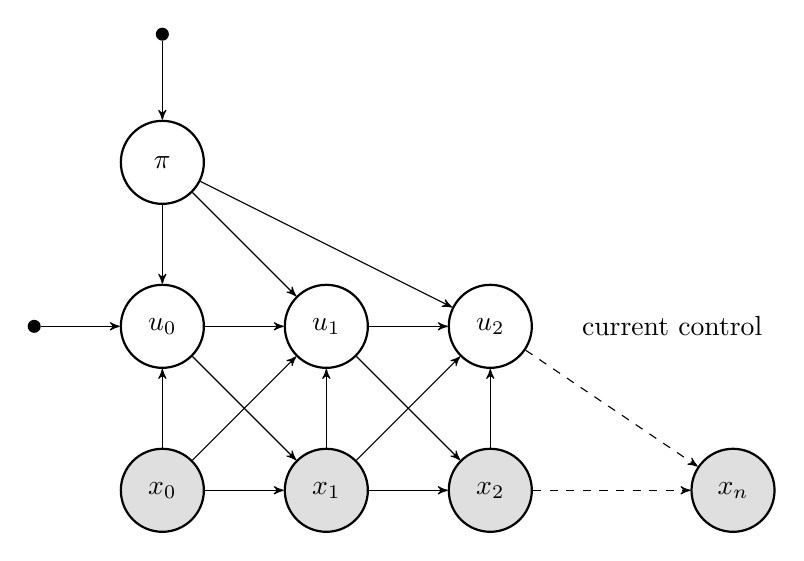
\begin{tikzpicture}

\tikzstyle{mylatent} = [circle,fill=white,draw=black,inner sep=1pt,
minimum size=30pt, thick]
\tikzstyle{myobs} = [circle,fill=gray!25,draw=black,inner sep=1pt,
minimum size=30pt, thick]

\node[mylatent] (u0) {$u_0$};
\node[mylatent, right=1 cm of u0] (u1) {$u_{1}$};
\node[mylatent, right=1 cm of u1] (u2) {$u_{2}$};
%\node[mylatent, right=2 cm of u2] (un) {$u_{n}$};

\node[myobs, below=1 cm of u0] (x0) {$x_0$};
\node[myobs, right=1 cm of x0] (x1) {$x_{1}$};
\node[myobs, right=1 cm of x1] (x2) {$x_{2}$};
\node[myobs, right=2 cm of x2] (xn) {$x_{n}$};

%\node[paramnode, left=1 cm of x0] (px0) {$$};
%\edge {px0} {x0}; 

\edge {x0} {x1};
\edge {x1} {x2}; 
\draw [dashed, ->] (x2) edge (xn);

\edge {u0} {x1}; 
\edge {u1} {x2}; 
\draw [dashed, ->] (u2) edge (xn);

\edge {x0} {u1}; 
\edge {x1} {u2}; 

\edge {u0} {u1}; 
\edge {u1} {u2}; 

\edge {x0} {u0}; 
\edge {x1} {u1}; 
\edge {x2} {u2}; 

\node[paramnode, left=1 cm of u0] (pu0) {$$};
\edge {pu0} {u0};

\node[mylatent, above=1 cm of u0] (policy) {$\pi$};

\edge {policy} {u0, u1, u2};

\node[paramnode, above=1 cm of policy] (ppolicy) {$$};
\edge {ppolicy} {policy};

\node [right=0.5cm of u2] {current control};

\end{tikzpicture}


}
\end{center}
Supervised learning of policy.\\
Full Bayesian treatment with Monte Carlo Variational Bayes.
\end{frame}

%%%%%%%%%%%%%%%%%%%%%%%%%%%%%%%%%%%%%%%%%%%%%%
\begin{frame}
\frametitle{Linear policy estimation}
Assumptions:
\begin{enumerate}
  \item control is linear w.r.t. some features (previous control, current speed, vector to the target, vector to the optimal trajectory, constant...)
  \item control noise is scaled with signal
\end{enumerate}

\end{frame}

\section{Min jerk trajectoy}

%%%%%%%%%%%%%%%%%%%%%%%%%%%%%%%%%%%%%%%%%%%%%%
\begin{frame}
\frametitle{Min jerk optimal trajectory}
Control cost:
\begin{align}
l(x, t) &= l(x^{(3)}, t) = x^{(3)}(t)^T W_i x^{(3)}(t) &&\text{cubic cost} \\
L(x) 	&= \int_0^T  l(x, t) dt = \int_0^T x^{(3)}(t)^T W_i x^{(3)}(t) &&\text{full cost} 
\end{align}

Boundary conditions: $x(0), x'(0), x(T), x'(T)$

\end{frame}

%%%%%%%%%%%%%%%%%%%%%%%%%%%%%%%%%%%%%%%%%%%%%%
\begin{frame}
\frametitle{Euler-Lagrange equation}
Find stationary solutions f the following functional:
\begin{align}
L(x) = \int_a^b l(t, x(t), x'(t)) dt
\end{align}

Optimal $x^*$ is a solution of the following Euler-Lagrange differential equation:
\begin{align}
\frac{\partial L}{\partial x} - \frac{d}{dt} \left( \frac{\partial L}{\partial x'} \right) = 0
\end{align}

When the functional depends on higher order derivatives
\begin{align}
L(x) = \int_a^b l(t, x(t), \{x^{(i)}(t), i \in 1 \ldots N\}) dt
\end{align}

the general form of the Euler-Lagrange equation is:
\begin{align}
\frac{\partial L}{\partial x} + \sum_{i=1}^N (-1)^N \frac{d}{dt} \left( \frac{\partial L}{\partial x^{(i)}} \right) = 0
\end{align}
\end{frame}


%%%%%%%%%%%%%%%%%%%%%%%%%%%%%%%%%%%%%%%%%%%%%%
\begin{frame}
\frametitle{Min jerk optimal trajectory}
Cost function reads:
\begin{align}
(x, t) &= l(x^{(3)}, t) = x^{(3)}(t)^T W_i x^{(3)}(t) &&\text{cubic cost} \\
L(x) 	&= \int_0^T  l(x, t) dt = \int_0^T x^{(3)}(t)^T W_i x^{(3)}(t) &&\text{full cost} 
\end{align}

Corresponding Euler-Lagrange equation is:
\begin{align}
2W_3x^{(6)}(t) = 0
\end{align}

which has a polynomial as a solution:
\begin{align}
x(t) &= a_5 t^5 + a_4 t^4 + a_3 t^3 + a_2 t^2 + a_1 t + a_0
\end{align}

\end{frame}

%%%%%%%%%%%%%%%%%%%%%%%%%%%%%%%%%%%%%%%%%%%%%%
\begin{frame}
\frametitle{Toy data}
\begin{center}
\includegraphics[width=0.7\textwidth]{./plots/toy/training.pdf}
\end{center}
Min-jerk trajectories with different boundary conditions
\end{frame}


%%%%%%%%%%%%%%%%%%%%%%%%%%%%%%%%%%%%%%%%%%%%%%
\begin{frame}
\frametitle{Toy data - sampling from the learned model}
\begin{center}
  \only<1> {\includegraphics[width=0.7\textwidth]{./plots/toy/disturbed-sampled-(1).pdf}}
  \only<2> {\includegraphics[width=0.7\textwidth]{./plots/toy/disturbed-sampled-(6).pdf}}
  \only<3> {\includegraphics[width=0.7\textwidth]{./plots/toy/disturbed-sampled-(15).pdf}}
\end{center}
\end{frame}




%%%%%%%%%%%%%%%%%%%%%%%%%%%%%%%%%%%%%%%%%%%%%%
\begin{frame}
\frametitle{Real data}
\begin{itemize}
  \item Too much variability
  \item No notion of global task in case of supervised policy learning
  \item Need contracting prior to constrain the policy space
\end{itemize}
\end{frame}


\end{document}